\section[The Pipeline]{Understanding the pipeline}
This section serves to represent our pipeline quantitatively and graphically. Table~\ref{tab:pipeline} showcases the data gathered by our pipeline, with the differential changes at each stage of the pipeline. 

At each stage of the pipeline, the amount of data trickles down, for instance, out of the \urls\ URLs we crawled, only \forms\ forms (\formsDelta) were found. Out of these, only \emailforms\ forms (\emailformsDelta) contained e-mail fields.

In our fuzzing attempts, the same behavior is repeated. We fuzzed \fuzzed\ forms with the regular payload, which resulted in a total of \recd\ e-mails (\recdDelta). After analysis of the received e-mails, we further fuzzed \fuzzed\ forms, which resulted in \success\ e-mails (\successDelta) which contain the vulnerability.
\begin{table}[!htbp]
	\centering
	\begin{tabular}{|c|l|c|c|}
		\hline
		\multicolumn{1}{|c|}{\textbf{S.No}} &
		\multicolumn{1}{c|}{\textbf{Pipeline Stage}} &
		\multicolumn{1}{p{3cm}|}{\centering \textbf{Quantity}} &
		\multicolumn{1}{p{2.8cm}|}{\centering \textbf{Differential}
		$\Delta$ d2/d1 * 100}\\
		\hline
		1 &  Crawled URLs  & \urls &  --- \\
		\hline
		2 &  Forms found  & \forms & \formsDelta \\
		\hline
		3 &  E-Mail Forms found  & \emailforms & \emailformsDelta \\
		\hline
		4 &  Fuzzed with regular payload  & \fuzzed & \fuzzedDelta \\
		\hline
		5 &  Received e-mails  & \recd & \recdDelta \\
		\hline
		6 &  Fuzzed with malicious payload  & \malfuzzed & \malfuzzedDelta \\
		\hline
		7 &  Successful attacks  & \success & \successDelta \\
		\hline

	\end{tabular}
	\caption[Data gathered by our pipeline]{Data gathered by our pipeline at each stage, with the differential between the stages.}
	\label{tab:pipeline}
\end{table}

\begin{figure}
	\centering
	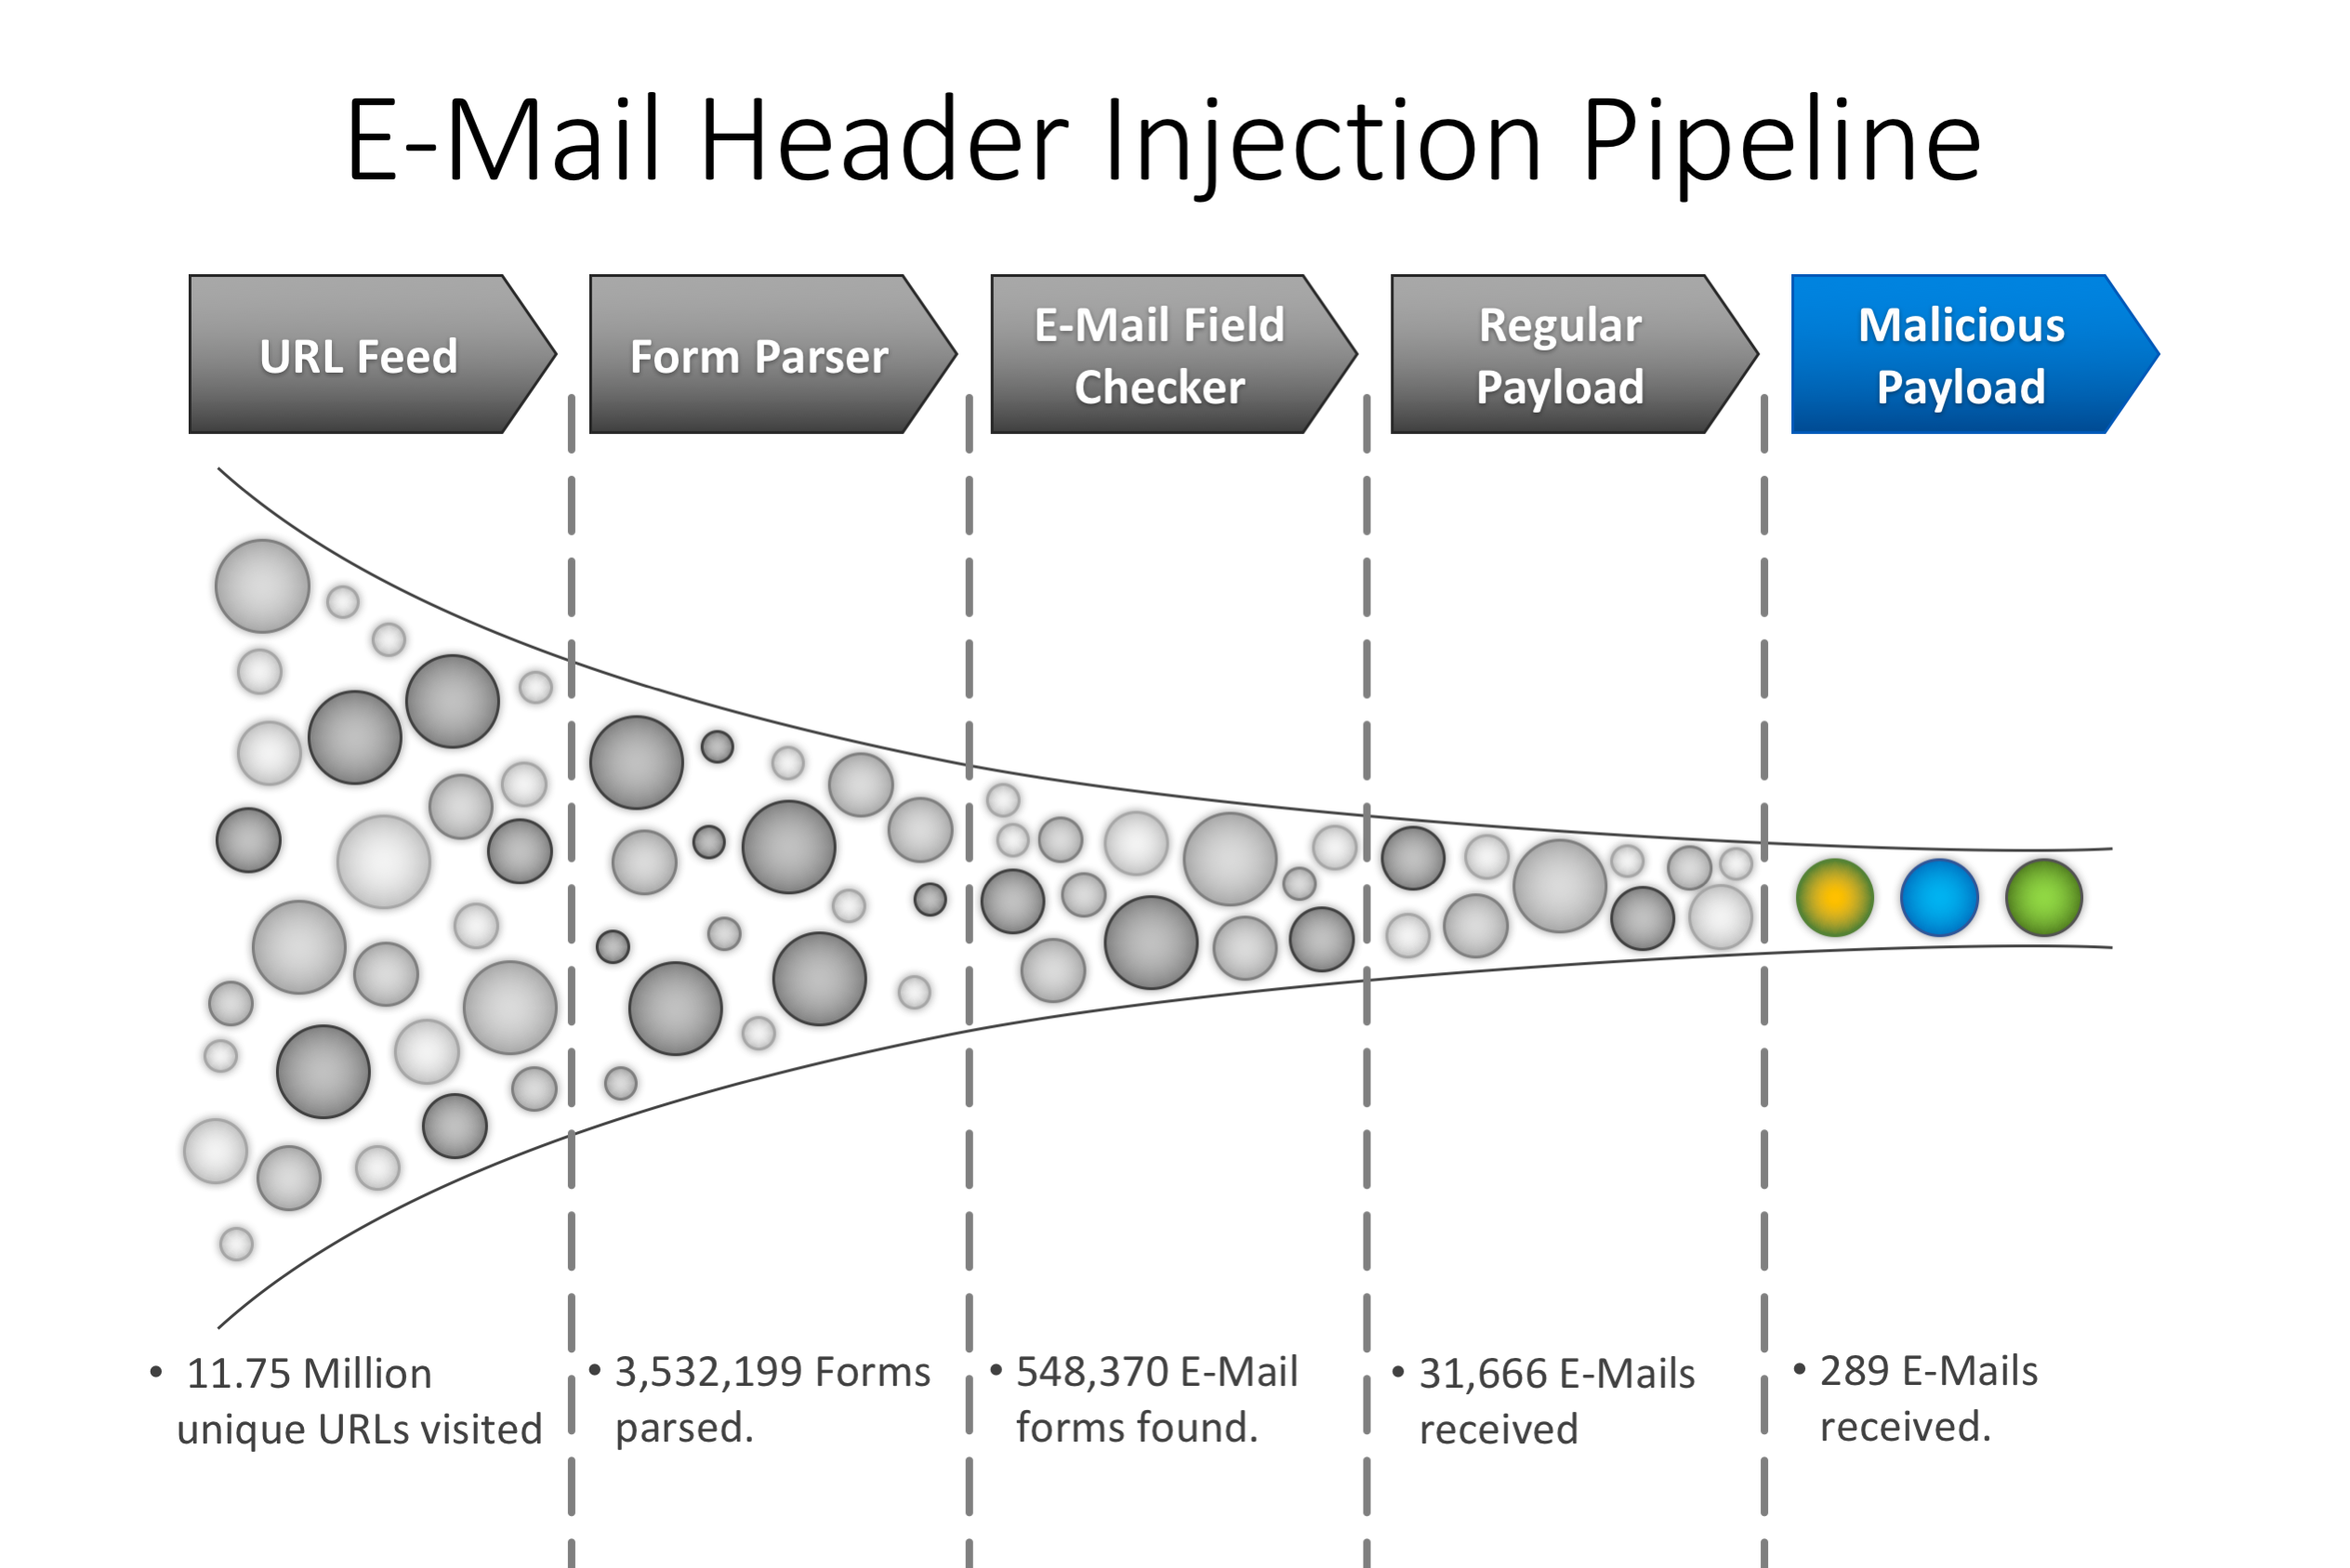
\includegraphics[width=16cm, height=9cm]{Results/emailheaderpipeline}
	\caption[\titlecap{E-Mail header injection Pipeline}]{Pipeline - shows the quantity of data gathered at each stage of the pipeline.}
	\label{fig:pipeline}
\end{figure}

Thus, our pipeline can be visualized as a funnel (shown in Figure~\ref{fig:pipeline}), where the quantity decreases until it reaches the end product.

From our research, it is clear that E-Mail Header Injection is quite widespread as a vulnerability, appearing on \successDelta\ of forms that we were able to perform automated attacks on. This value acts as a lower bound for E-Mail Header Injection vulnerability, and can quite easily be much more if the attacks were of a more concentrated nature, crafted for the individual websites and less automated. We discuss this possibility, and other concepts such as limitations in the following chapter.